In Section \ref{sub:tridual} we mentioned that we would like $\pi$ to be the piecewise linear analogue to the generic proper smooth map of Section \ref{sec:3bound4}.
The important condition that we do not necessarily have is genericity.
An investigation of the analogue to critical points of $\pi$ demonstrates why an appropriate choice of edge blowups will introduce the genericity we are looking for.

Generic singular fibers in the smooth case have the form of either a point or a figure 8 graph.
Taking $T$, $\pi:T\to\C$, and $X$ be as in Section \ref{sub:tridual}.
A singular fiber of a $\pi$ is found by checking how simplicial circles change when we pass over the images of edges in $T$.
Let $X(c_i)$, $X(c_j)$ be 2--cells in $X$ that intersect at a 1--cell $X(e)$, let $c_i$, $c_j$ be the regions of points of type 5 in the plane corresponding to $X(c_i)$, $X(c_j)$, and let $e$ be the strand of points of type 4 that corresponds to $X(e)$.
Let $E$ be the edge of $T$ with $e\subset\pi(E)$, let $C_i=\{C_{i,k}\}$ be the collection of simplicial circles in $T^*$ that correspond to the circles of $T$ that map through $\pi$ over $c_i$, and let $C_j=\{C_{j,l}\}$ be the similar collection for $c_j$.
Considering $C_i$ and $C_j$ as sets of edges in $T^*$, the method of building $C_i$ and $C_j$ found in Algorithm \ref{alg:regularcircles} tells us that the symmetric difference of $C_i$ and $C_j$ is either the boundary of the dual 2--cell $E*$, or is empty.

The form of the singular fiber over a point in $e$ is then seen by pulling the centres of the edges of $\pd E^*$ towards the centre of $E^*$.
This is justified by considering the centre of $E^*$ as the sole intersection of $E$ and $E^*$, and recognizing that the preimage of a point in $e$ through $\pi$ must intersect the edge $E$.
We illustrate this situation in Figure \ref{fig:plsingularities}.

\begin{figure}
	\centering
	\captionsetup{justification=centering}
	\caption{Simplicial circles near an edge}
	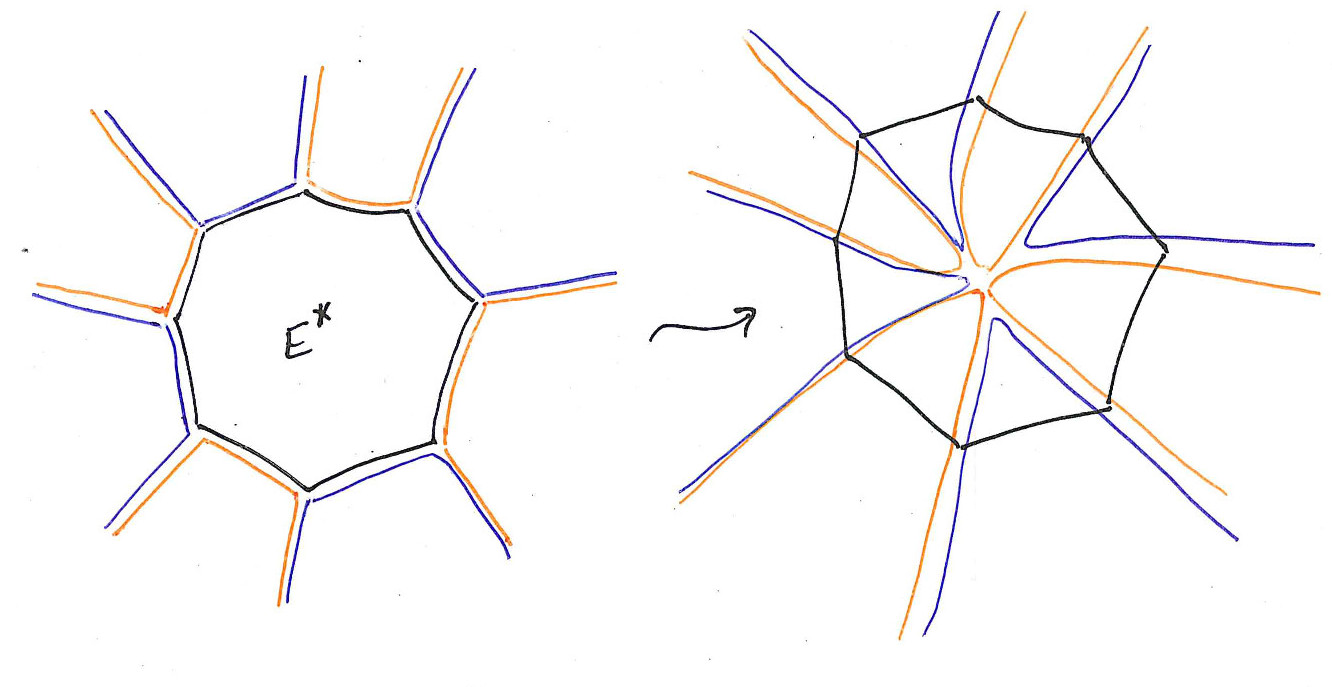
\includegraphics[height=3in]{figures/plsingularities.jpg}
	\label{fig:plsingularities}
\end{figure}

The form of the singular fiber is then the wedge of $n$ simplicial circles.
We define $n$ to be the \emph{wedge number} of $E$, and this can be computed by investigating the link of $E$ in $T$ through $\pi$, which is precisely what we do in Algorithm \ref{alg:computewedgenum}.

\begin{algorithm}
	\caption{Wedge number computations}
	\label{alg:computewedgenum}
	\KwData{$T$, $\pi:T\to\C$, and edge $E$ of $T$}
	\KwResult{the wedge number of $E$, denoted $w_E$}
	\Begin{
		$C\longleftarrow\lk{E}=\{e_0,e_1,\dots,e_k,e_0\}$ as a cycle of the graph $T^1$\;
		$w_E\longleftarrow 0$\;
		\ForEach{edge $e$ in $C$}{
			\If{$\pi(e)$ crosses $\pi(E)$}{
				$w_E\longleftarrow w_E+1/2$\;
			}
		}
	}
\end{algorithm}

Using the fact that $T$ is closed, we get that $\lk{E}$ is a simplicial circle in the 1--skeleton of $T$.
Because $\pi$ maps the vertices of these circles to $S^1\subset\C$, we classify the edges in $\lk{E}$ into those that pass over $e=\pi(E)$ and those that do not.
There is an even number of edges that cross $e$ because $\lk{E}$ is closed.
An edge $F$ of $\lk{E}$ with $f=\pi(F)$ crossing $e$ determines uniquely a tetrahedron $\sigma$ with $F,E\in\sigma^1$.
For $x_i\in c_i$ and $x_j\in c_j$, take $\gamma$ to be a simple path from $x_i$ to $x_j$ that crosses $e$ transversely exactly once.
Then $\pi\inv(x_i)$ and $\pi\inv(x_j)$ each intersect $\sigma$, and the preimage of every point in $\gamma$ does so as well.
A representative of this situation is seen in Figure \ref{fig:gammapullback}.
To turn $\pi\inv(x_i)$ into $\pi\inv(x_j)$ along $\gamma$, the simplicial circle passes through $\sigma$ and over $E$.

\begin{figure}
	\centering
	\captionsetup{justification=centering}
	\caption{Preimages of points on either side of $e$ as they sit in $\sigma$}
	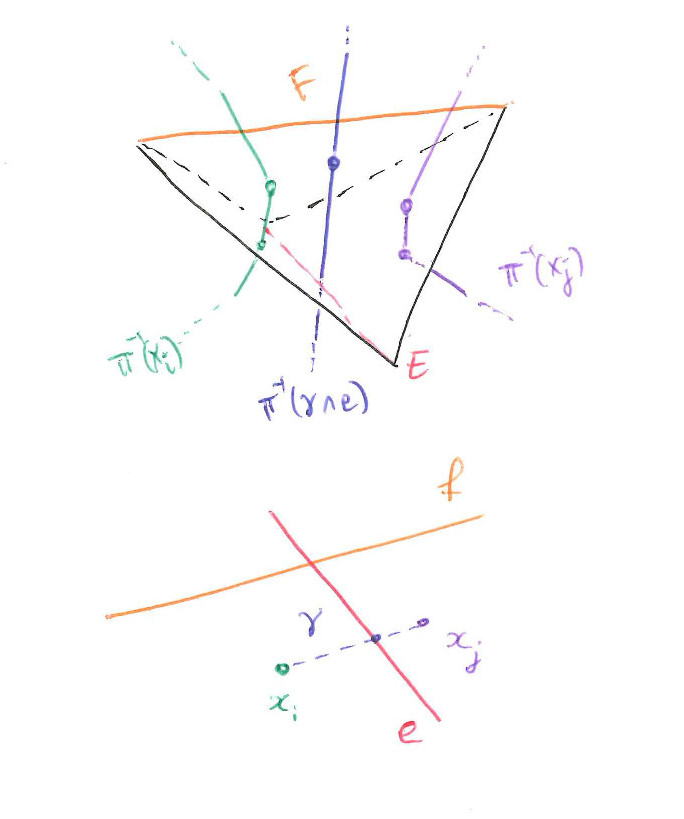
\includegraphics[width=3.75in]{figures/gammapullback.jpg}
	\label{fig:gammapullback}
\end{figure}

The edges of $\lk{E}$ that do not cross $e$ determine tetrahedra that do not have this property.
Each edge of $\lk{E}$ that crosses $e$ then contributes one half of one circle in the bouquet of circles that map over $e$, hence contributes $+1/2$ to the computation of the wedge number.

We strive for the piecewise analogue of genericity and this happens when the wedge number of each edge in $T$ is 0, 1, or 2.
One way to achieve this is through the use of edge blowups.
In order to perform edge blowups, we modify our triangulation to a truncated triangulation.
Truncating in this way and then performing edge blowups makes tracking data through edges more trouble than its worth, and leads to confusion.
Instead, we turn to the dual decomposition for a better way.

We keep $T$ as our 3--manifold triangulation and $T^*$ as its dual.
Let $E$ be an edge of $T$ with dual 2--cell of $E^*$.
The computation of a wedge number for $E$ assigned each edge in $\lk{E}$ a contributing coefficient of $0$ or $+1/2$.
In the justification of this assignment, it was demonstrated that the contribution comes from the tetrahedrons uniquely determined by the edges of $\lk{E}$ rather than the edges themselves.
For each edge $E$ of $T$ (2--cell $E^*$ of $T^*$), the tetrahedra containing $E$ (the vertices in the boundary of $E^*$) are assigned a wedge coefficient of 0 or $+1/2$.
The wedge number for $E$ ($E^*$) is then computed as the sum of the wedge coefficients surrounding it.

Recall that the modification to $T^*$ equivalent to an edge blowup was the splitting of a 2--cell by a new edge.
In the view from $T$, the 3--cells over which we blowup still contain and map over each of the new edges, while the remaining 2--cells contain only one of the edges.
The 3--cells over which we split then contribute to the wedge numbers of both edges, while the rest contribute to only one.

In $T^*$, we have split a 2--cell by a 1--cell connecting a pair of vertices.
The vertices over which we connect contribute their wedge coefficient to both of the new 2--cells because the corresponding 3--cells project over both of the new edges.
The wedge numbers of the new 2--cells are then easily recomputed as displayed in Figure \ref{fig:wedgenumblowup}.
The details to reduce a single edge number are found in Algorithm \ref{alg:wedgereduction}

\begin{algorithm}
	\caption{Wedge number reduction}
	\label{alg:wedgereduction}
	\KwData{a dual 2--cell $E^*$ of a truncated dual complex $T'^*$ with wedge number $w_E>2$}
	\KwResult{a pair of dual vertices $(\sigma^*,\tau^*)$ of $\pd E^*$ over which we may split $E^*$, so that the two new 2--cells have wedge numbers of 2 and $w_E-1$}
	\Begin{
		$C\longleftarrow\pd E^*=\{\sigma_0^*,\dots,\sigma_k^*\}$ as a cycle in the 1--skeleton of $T'^*$\;
		$\sigma^*\longleftarrow\sigma_i^*$ where $\sigma_i^*$ is the first dual vertex in $C$ with nonzero wedge coefficient\;
		$w,j\longleftarrow 0$\;
		\While{$w<2$}{
			$j\longleftarrow j+1$\;
			$c_j\longleftarrow$ the wedge coefficient of the dual vertex $\sigma_{i+j}^*$\;
			$w\longleftarrow w+c_j$\;			
		}
		$\tau^*\longleftarrow \sigma_{i+j}^*$\;
	}
\end{algorithm}

\begin{figure}
	\centering
	\captionsetup{justification=centering}
	\caption{Wedge numbers after a blowup}
	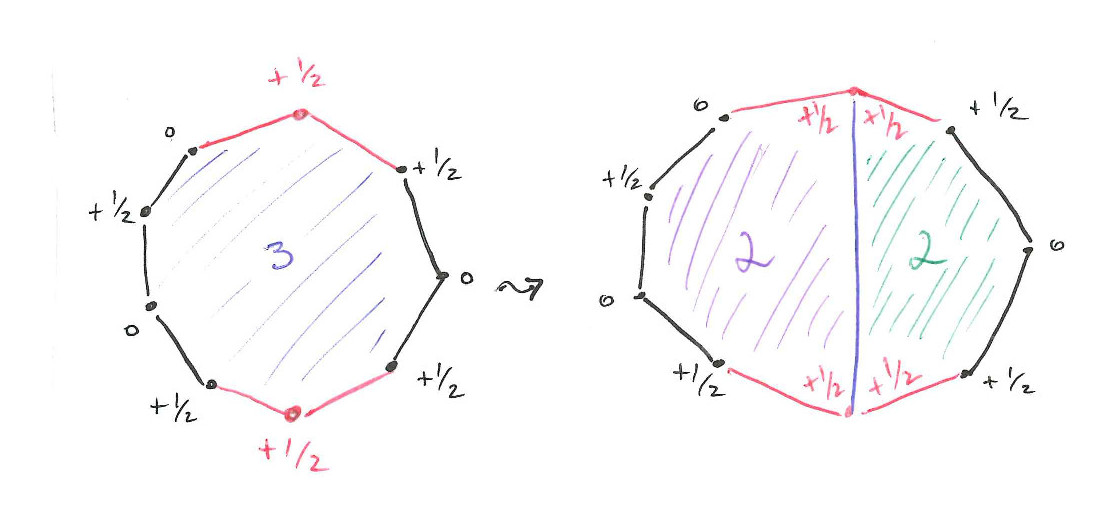
\includegraphics[width=5.5in]{figures/wedgenumblowup.jpg}
	\label{fig:wedgenumblowup}
\end{figure}